% Figures of the paper; data from fig/make_figdata.py. Colours: categorical slot 1 blue 2A78D6, slot 2 orange EB6834,
% slot 3 aqua 1BAF7A; text and axes in grey ink.
\definecolor{cblue}{HTML}{2A78D6}
\definecolor{corange}{HTML}{EB6834}
\definecolor{caqua}{HTML}{1BAF7A}
\definecolor{cink}{HTML}{52514E}
\definecolor{cgrid}{HTML}{D9D8D3}

% the tube: sections at t = 0.05, 0.25, 0.5, 0.75, 0.95 (fig/make_tube.py), light to dark in time
\definecolor{ct0}{HTML}{9EC5F4}
\definecolor{ct1}{HTML}{6DA7EC}
\definecolor{ct2}{HTML}{3987E5}
\definecolor{ct3}{HTML}{256ABF}
\definecolor{ct4}{HTML}{184F95}
\newcommand{\figtube}{%
\begin{tikzpicture}
\begin{axis}[width=0.8\textwidth, height=0.62\textwidth, xmin=-15, xmax=82, ymin=-12, ymax=78,
  xlabel={longitude (deg)}, ylabel={latitude (deg)}, axis line style={cink}, tick style={cink},
  label style={cink, font=\small}, tick label style={cink, font=\footnotesize}, grid=major,
  grid style={cgrid, very thin}, clip=true]
\addplot[ct0, line width=0.9pt] table {fig/fig_tube_t0.dat};
\addplot[ct1, line width=0.9pt] table {fig/fig_tube_t1.dat};
\addplot[ct2, line width=0.9pt] table {fig/fig_tube_t2.dat};
\addplot[ct3, line width=0.9pt] table {fig/fig_tube_t3.dat};
\addplot[ct4, line width=0.9pt] table {fig/fig_tube_t4.dat};
\addplot[corange, line width=1pt, dashed] coordinates {(60,-12) (60,78)};
\addplot[cink, line width=1.4pt] table {fig/fig_shape_twelfth.dat};
\addplot[only marks, mark=*, mark size=1.8pt, cink] table {fig/fig_tube_eight.dat};
\addplot[only marks, mark=x, mark size=3.5pt, line width=1pt, cink] coordinates {(60,0)};
\addplot[only marks, mark=*, mark size=2.2pt, caqua] coordinates {(0,0)};
\node[font=\footnotesize, caqua, anchor=north east] at (axis cs:-1,-1) {$E$};
\node[font=\footnotesize, corange, anchor=west] at (axis cs:61,72) {$I$};
\node[font=\footnotesize, cink, anchor=north west] at (axis cs:61,-1) {$C_{23}$};
\node[font=\footnotesize, ct0, anchor=west] at (axis cs:10.5,-6) {$t=0.05$};
\node[font=\footnotesize, ct4, anchor=west] at (axis cs:66,30) {$t=0.95$};
\end{axis}
\end{tikzpicture}}

\newcommand{\figshape}{%
\begin{tikzpicture}
\begin{axis}[width=0.95\textwidth, height=0.46\textwidth, xmin=-180, xmax=180, ymin=-90, ymax=90,
  xtick={-180,-120,-60,0,60,120,180}, ytick={-90,-45,0,45,90}, xlabel={longitude (deg)}, ylabel={latitude (deg)},
  axis line style={cink}, tick style={cink}, label style={cink, font=\small}, tick label style={cink, font=\footnotesize},
  grid=major, grid style={cgrid, very thin}, clip=true]
\foreach \i in {0,...,10} {\addplot[cink!45, line width=0.6pt] table {fig/fig_shape_copy\i.dat};}
\addplot[cblue, line width=1.6pt] table {fig/fig_shape_twelfth.dat};
% the plane I: meridians 60 and -120 deg
\addplot[corange, line width=1pt, dashed] coordinates {(60,-90) (60,90)};
\addplot[corange, line width=1pt, dashed] coordinates {(-120,-90) (-120,90)};
% collisions (equator at 180, 60, -60) and Euler points (0, 120, -120)
\addplot[only marks, mark=x, mark size=3.5pt, line width=1pt, cink] coordinates {(180,0) (-180,0) (60,0) (-60,0)};
\addplot[only marks, mark=*, mark size=2.2pt, caqua] coordinates {(0,0) (120,0) (-120,0)};
\node[font=\footnotesize, cblue, anchor=south east] at (axis cs:28,22) {$\gamma_8$};
\node[font=\footnotesize, caqua, anchor=north] at (axis cs:0,-5) {$E$};
\node[font=\footnotesize, corange, anchor=west] at (axis cs:62,70) {$I$};
\node[font=\footnotesize, cink, anchor=north] at (axis cs:60,-5) {$C_{23}$};
\end{axis}
\end{tikzpicture}}

\newcommand{\figlogic}{%
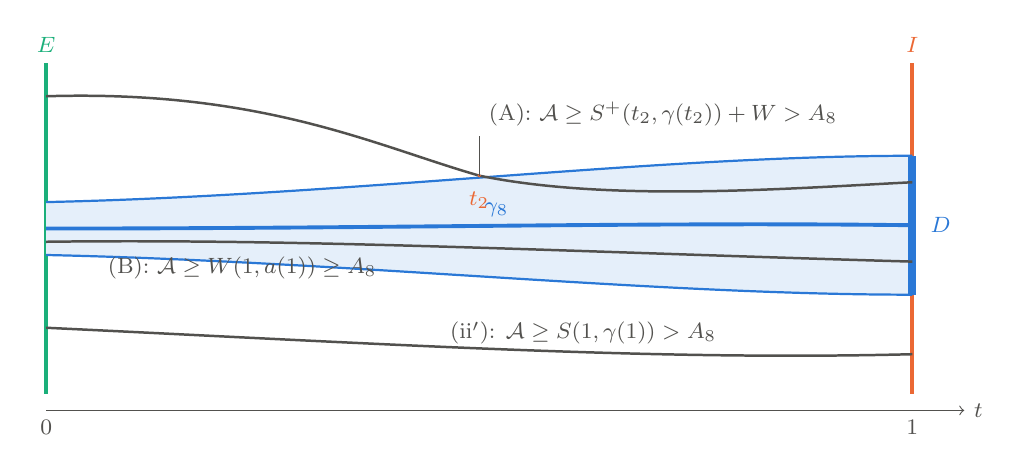
\begin{tikzpicture}[x=11cm, y=4.2cm, font=\footnotesize]
% axes: time 0 (E) to 1 (I)
\draw[cink, ->] (0,-0.05) -- (1.06,-0.05) node[right] {$t$};
\node[cink, below] at (0,-0.05) {$0$}; \node[cink, below] at (1,-0.05) {$1$};
\draw[caqua, line width=1.4pt] (0,0) -- (0,1) node[above] {$E$};
\draw[corange, line width=1.4pt] (1,0) -- (1,1) node[above] {$I$};
% the tube (closed label sets mapped forward), its end disc D on I
\fill[cblue!12] (0,0.42) .. controls (0.35,0.40) and (0.7,0.30) .. (1,0.30) -- (1,0.72)
  .. controls (0.7,0.72) and (0.35,0.60) .. (0,0.58) -- cycle;
\draw[cblue, line width=0.8pt] (0,0.42) .. controls (0.35,0.40) and (0.7,0.30) .. (1,0.30);
\draw[cblue, line width=0.8pt] (0,0.58) .. controls (0.35,0.60) and (0.7,0.72) .. (1,0.72);
\draw[cblue, line width=3pt] (1,0.30) -- (1,0.72);
\node[cblue, right] at (1.01,0.51) {$D$};
% the eight
\draw[cblue, line width=1.4pt] (0,0.5) .. controls (0.4,0.5) and (0.7,0.52) .. (1,0.51);
\node[cblue, above] at (0.52,0.505) {$\gamma_8$};
% (B): stays in the tube, starts on E
\draw[cink, line width=0.9pt] (0,0.46) .. controls (0.3,0.47) and (0.6,0.43) .. (1,0.40);
\node[cink, anchor=west] at (0.06,0.38) {(B): $\mathcal A\ge W(1,a(1))\ge A_8$};
% (A): leaves the tube; last exit t_2
\draw[cink, line width=0.9pt] (0,0.9) .. controls (0.25,0.92) and (0.38,0.75) .. (0.5,0.66)
  .. controls (0.65,0.58) and (0.85,0.62) .. (1,0.64);
\fill[corange] (0.5,0.66) circle (0.6pt);
\node[cink, anchor=south west] at (0.5,0.78) {(A): $\mathcal A\ge S^+(t_2,\gamma(t_2))+W>A_8$};
\draw[cink, very thin] (0.5,0.66) -- (0.5,0.78);
\node[corange, anchor=north] at (0.5,0.64) {$t_2$};
% (ii'): ends on I outside D
\draw[cink, line width=0.9pt] (0,0.2) .. controls (0.4,0.15) and (0.7,0.1) .. (1,0.12);
\node[cink, anchor=south] at (0.62,0.12) {(ii$'$): $\mathcal A\ge S(1,\gamma(1))>A_8$};
\end{tikzpicture}}

\newcommand{\figcover}{%
\begin{tikzpicture}
\begin{axis}[width=0.9\textwidth, height=0.5\textwidth, xmin=0.37, xmax=1.32, ymin=-3.3, ymax=1.55,
  xlabel={$\theta$}, ylabel={$\kappa=M/\sqrt{\varepsilon}$}, axis line style={cink}, tick style={cink},
  label style={cink, font=\small}, tick label style={cink, font=\footnotesize},
  colormap={eps}{HTML(0cm)=(CDE2FB); HTML(1cm)=(9EC5F4); HTML(2cm)=(6DA7EC); HTML(3cm)=(3987E5);
    HTML(4cm)=(256ABF); HTML(5cm)=(184F95); HTML(6cm)=(0D366B)},
  point meta min=-3, point meta max=-0.699, colorbar, colorbar style={ylabel={$\log_{10}\varepsilon_{\rm top}$},
  ylabel style={cink, font=\footnotesize}, tick label style={cink, font=\footnotesize}, width=0.25cm}]
\addplot graphics[xmin=0.37, xmax=1.32, ymin=-3.3, ymax=1.55] {fig/fig_cover.png};
\end{axis}
\end{tikzpicture}}

\newcommand{\figcellmin}{%
\begin{tikzpicture}
\begin{semilogyaxis}[width=0.9\textwidth, height=0.42\textwidth, xmin=-3.2, xmax=11.2,
  xlabel={$\sigma$ (cell layer)}, ylabel={$\min F$ per cell},
  axis line style={cink}, tick style={cink}, label style={cink, font=\small},
  tick label style={cink, font=\footnotesize}]
\addplot[name path=hi, draw=none, forget plot] table[x=sigma, y=fmax] {fig/fig_cellmin_layers.dat};
\addplot[name path=lo, draw=none, forget plot] table[x=sigma, y=fmin] {fig/fig_cellmin_layers.dat};
\addplot[cblue!15, forget plot] fill between[of=hi and lo];
\addplot[cblue, line width=1.2pt] table[x=sigma, y=fmin] {fig/fig_cellmin_layers.dat};
\addplot[cink, line width=0.8pt, dashed] table[x=sigma, y=fmed] {fig/fig_cellmin_layers.dat};
\end{semilogyaxis}
\end{tikzpicture}}
